% magick -quality 90 -density 1200 $input -resize 25% -trim $output

\documentclass{standalone}
\usepackage{tikz}

\usetikzlibrary{math}


\begin{document}

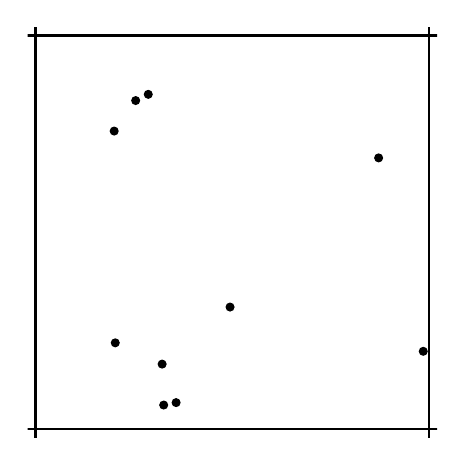
\begin{tikzpicture}
  \path[clip] (-0.1,-0.1) rectangle (5.1, 5.1);
  \draw[thick] (-1,0) -- (6,0);
  \draw[thick] (-1,5) -- (6,5);
  \draw[thick] (0,-1) -- (0,6);
  \draw[thick] (5,-1) -- (5,6);

  \foreach \i in {1,...,10} {
    \tikzmath{
      real \x;
      real \y;
      \x = random() * 5;
      \y = random() * 5;
    }
    \draw[fill=black] (\x,\y) circle [radius=0.05cm];
  }
\end{tikzpicture}

\end{document}